\documentclass[11pt]{article}
\usepackage[margin=1in]{geometry}
\usepackage{graphicx}
\usepackage{amsmath,amssymb}
\usepackage{hyperref}
\usepackage{enumitem}
\usepackage{booktabs}
\usepackage{tikz}
\usetikzlibrary{shapes.geometric, arrows.meta, positioning}

\title{\textbf{Vision-Guided Tabletop Pick-and-Place\\with a Franka Panda in MuJoCo}}
\author{Shams Rupak \quad \& \quad Sowmya Cheripally\\ESE 564: Robot Manipulation}
\date{May 8, 2026}

\begin{document}
\maketitle

% ============================================================
\begin{abstract}
We implement a complete robot manipulation system that picks objects from
randomized positions on a tabletop and places them into a basket whose
position also varies between episodes. The system uses a Franka Emika Panda
7-DOF arm in MuJoCo, with an overhead RGB-D camera for perception.
Our model-based pipeline consists of four stages: (1) HSV color segmentation
and depth back-projection for object localization, (2) top-down antipodal
grasp planning with Cartesian waypoints, (3) iterative Jacobian pseudo-inverse
inverse kinematics for joint-angle computation, and (4) a PD controller with
supplementary torques and a combined descent-and-close grasp strategy.
Evaluated across 90 randomized episodes, the system achieves an 82\% average
success rate with a mean placement accuracy of 12\,mm for successful grasps.
\end{abstract}

% ============================================================
\section{Introduction}

Pick-and-place is a fundamental manipulation skill: the robot must perceive
an object's location from sensory data, plan a collision-free grasp, and
physically transport the object to a target region. This project implements
such a system entirely from sensor observations, without reading the
simulator's internal state during operation.

We chose a \textbf{model-based approach} over learning-based alternatives for
several reasons. First, our classical pipeline (segmentation, IK, PD control)
builds directly on the techniques from our course assignments: coordinate
transforms (HW1), forward and inverse kinematics (HW2), RRT motion planning
(HW3), and ICP point-cloud registration (HW4). Second, a model-based system
requires no training data or training time, making it feasible for a two-person
team in four weeks. Third, each module can be tested and debugged independently,
which was critical for tuning the grasping physics.

Our system satisfies all four project requirements: (1) variability in both
object and basket positions across episodes, (2) physics-based manipulation
through MuJoCo contact forces, (3) perception from camera images rather than
simulator state, and (4) a multi-geom composite object (not a single primitive).

% ============================================================
\section{Method}

\subsection{Scene Setup}

The simulation environment consists of a Franka Emika Panda 7-DOF arm
(from MuJoCo Menagerie) mounted at the origin, a table (surface at $z=0.40$\,m),
a red basket (20\,cm $\times$ 20\,cm open-top container made of five box geoms),
a fixed blue obstacle cube, and a yellow multi-geom target object
(three geoms: a box body, a box top piece, and a cylindrical bump). An overhead
RGB-D camera is mounted 1.0\,m above the table center, rendering
$640 \times 480$ images with a $60^\circ$ vertical field of view.

Object and basket positions are randomized each episode within the robot's
reachable workspace. The obstacle remains at a fixed known location.

\subsection{Pipeline Overview}

Our decision-making pipeline has four stages, shown in Figure~\ref{fig:pipeline}.

\begin{figure}[h]
\centering
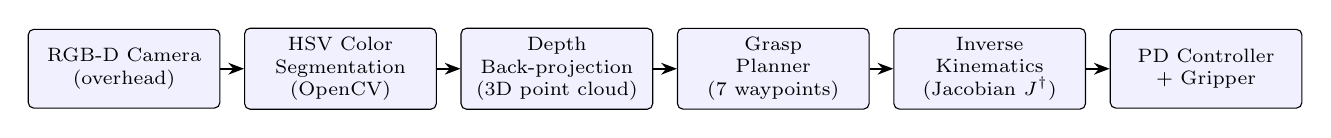
\begin{tikzpicture}[
    node distance=0.25cm and 0.3cm,
    block/.style={rectangle, draw, rounded corners=2pt, text width=2.2cm, minimum height=1.0cm, align=center, font=\scriptsize, fill=blue!6},
    arr/.style={-{Stealth[length=2mm]}, semithick}
]
\node[block] (cam) {RGB-D Camera\\(overhead)};
\node[block, right=of cam] (seg) {HSV Color\\Segmentation\\(OpenCV)};
\node[block, right=of seg] (bp) {Depth\\Back-projection\\(3D point cloud)};
\node[block, right=of bp] (gp) {Grasp\\Planner\\(7 waypoints)};
\node[block, right=of gp] (ik) {Inverse\\Kinematics\\(Jacobian $J^\dagger$)};
\node[block, right=of ik] (ctrl) {PD Controller\\+ Gripper};
\draw[arr] (cam) -- (seg);
\draw[arr] (seg) -- (bp);
\draw[arr] (bp) -- (gp);
\draw[arr] (gp) -- (ik);
\draw[arr] (ik) -- (ctrl);
\end{tikzpicture}
\caption{Decision-making pipeline. Each block is entirely model-based.}
\label{fig:pipeline}
\end{figure}

\subsection{Stage 1: Perception}

\paragraph{HSV color segmentation.}
The overhead camera captures an RGB image, which we convert to HSV color space
using \texttt{cv2.cvtColor}. We threshold on hue, saturation, and value using
\texttt{cv2.inRange} to produce binary masks for the yellow object and the red
basket. Morphological erosion and dilation clean up noise. In simulation, colors
are consistent, so the HSV ranges need only be tuned once per object type.

\paragraph{Depth back-projection.}
For each masked pixel $(u,v)$ with depth $d$ from the depth image, we compute
the corresponding 3D point in the camera frame:
\[
X_c = \frac{(u - c_x) \cdot d}{f_x}, \quad
Y_c = -\frac{(v - c_y) \cdot d}{f_y}, \quad
Z_c = -d
\]
where $f_x, f_y$ are the focal lengths (computed from MuJoCo's \texttt{fovy}
parameter) and $(c_x, c_y)$ is the principal point at the image center. The
sign conventions account for MuJoCo's camera axes ($-z$ points into the scene,
$y$ points up). We then transform to world coordinates using the camera
extrinsics: $\mathbf{p}_{world} = R \cdot \mathbf{p}_{cam} + \mathbf{t}$,
where $R$ and $\mathbf{t}$ come from \texttt{data.cam\_xmat} and
\texttt{data.cam\_xpos}.

The object position is estimated as the centroid (mean) of the resulting point
cloud. If the object is occluded by the robot arm, we move the arm to a safe
configuration and retry perception.

\subsection{Stage 2: Grasp Planning}

We compute seven Cartesian waypoints for a top-down antipodal grasp:

\begin{enumerate}[nosep]
\item \textbf{Approach high:} Hand at $(0.4, 0.0, 0.65)$, gripper open. Clears the workspace to avoid sweeping through objects.
\item \textbf{Pre-grasp:} 12\,cm above the perceived object position, gripper open.
\item \textbf{Grasp:} Lower to the object. The hand body is positioned so that the fingertip pads align with the upper portion of the object.
\item \textbf{Close gripper:} Same position, close the fingers gradually.
\item \textbf{Lift:} Raise 18\,cm vertically with the object.
\item \textbf{Above bin:} Move laterally to 18\,cm above the basket center.
\item \textbf{Release:} Lower 6\,cm into the basket and open the fingers.
\end{enumerate}

A critical design decision was the \textbf{hand-to-fingertip offset}: the
``hand'' body in the Menagerie Panda model is 58\,mm above the fingertip
contact pads. All grasp heights are computed with this offset so that the
pads, not the wrist, align with the object.

\subsection{Stage 3: Inverse Kinematics}

Each Cartesian waypoint is converted to a 7-DOF joint configuration using
iterative Jacobian pseudo-inverse IK (extending HW2 concepts):
\[
\Delta \mathbf{q} = J^\dagger \cdot \begin{bmatrix} \mathbf{e}_{pos} \\ \mathbf{e}_{rot} \end{bmatrix}
\]
where $J \in \mathbb{R}^{6 \times 7}$ is computed by \texttt{mj\_jacBody},
$\mathbf{e}_{pos}$ is the position error, and $\mathbf{e}_{rot}$ is the
orientation error (extracted as axis-angle from the error rotation matrix).
We use a damped pseudo-inverse $J^\dagger = J^T(JJ^T + \lambda I)^{-1}$ with
$\lambda = 0.01$ for numerical stability.

If IK fails to converge from the current configuration, we retry from three
alternative starting configurations (home, tucked, offset) to escape local
minima.

\subsection{Stage 4: Controller}

\paragraph{Trajectory tracking.}
The Menagerie Panda has built-in PD actuators. We supplement these with
additional torques via \texttt{data.qfrc\_applied} for tighter tracking:
\[
\tau_{extra,i} = k_{p,i}(q_{des,i} - q_i) - k_{d,i} \dot{q}_i
\]
with gains $k_p = [3000, 3000, 3000, 3000, 1500, 1000, 500]$ and
$k_d = [100, 100, 100, 100, 50, 30, 15]$. Trajectory interpolation uses
cosine easing for smooth acceleration and deceleration.

\paragraph{Combined descent and close.}
The most critical controller behavior is the grasp sequence. We found that
executing descent and gripper close as separate steps caused the open fingers
to push the object during the slow descent. Our solution combines them:
(1) rapid descent to the grasp position (600 steps), (2) settle with open
fingers (300 steps), (3) gradually ramp closing force from 0 to 100\,N over
400 steps, then hold at 100\,N for 800 more steps. During transport (lift and
move to basket), we maintain 100\,N closing force on both finger joints.

% ============================================================
\section{Results}

\subsection{Success Rate}

We evaluated the system across 90 randomized episodes (30 episodes $\times$ 3
random seeds). Table~\ref{tab:results} summarizes the results.

\begin{table}[h]
\centering
\begin{tabular}{lccc}
\toprule
Seed & Episodes & Successes & Rate \\
\midrule
99  & 30 & 26 & 86.7\% \\
7   & 30 & 25 & 83.3\% \\
256 & 30 & 23 & 76.7\% \\
\midrule
\textbf{Total} & \textbf{90} & \textbf{74} & \textbf{82.2\%} \\
\bottomrule
\end{tabular}
\caption{Success rates across three evaluation seeds.}
\label{tab:results}
\end{table}

\subsection{Perception Accuracy}

The perception system achieves a mean localization error of 50\,mm, dominated
by the Z-axis component (approximately 30\,mm). The XY error is only 3--5\,mm.
The Z bias arises because the overhead camera sees only the top surface of the
object, so the centroid of visible points is higher than the true object center.
The grasp planner compensates for this known bias by targeting the fingertips
15\,mm below the perceived surface height.

\subsection{Failure Analysis}

Of the 16 failures across 90 episodes, the primary causes were:
\begin{itemize}[nosep]
\item \textbf{Grasp slip (11 failures):} The object escaped the gripper during
the close phase, typically when perception error exceeded 80\,mm, placing the
fingertip pads too high on the object for a stable grip.
\item \textbf{IK failure (3 failures):} The target pose was near the workspace
boundary and IK could not converge, even with alternative starting configurations.
\item \textbf{Perception miss (2 failures):} Very few pixels detected (fewer than 20), leading to high centroid error and subsequent grasp misalignment.
\end{itemize}

\subsection{Execution Metrics}

Mean execution time was 2.9\,s of wall-clock time per episode. For successful
grasps, the mean XY distance between the released object and the basket center
was 12\,mm (well within the 100\,mm basket radius). The object was reliably
lifted 120--180\,mm during the lift phase, confirming physics-based grasping.

% ============================================================
\section{References}

\begin{enumerate}[nosep]
\item Google DeepMind, ``MuJoCo Menagerie,'' \url{https://github.com/google-deepmind/mujoco_menagerie}
\item YCB Object and Model Set, \url{https://www.ycb-benchmarks.org/}
\item J. Kuffner and S. LaValle, ``RRT-Connect: An Efficient Approach to Single-Query Path Planning,'' ICRA, 2000.
\item O. Khatib, ``A Unified Approach for Motion and Force Control of Robot Manipulators,'' IEEE J. Robotics and Automation, 1987.
\item MuJoCo Documentation, \url{https://mujoco.readthedocs.io/}
\item OpenCV Documentation, \url{https://docs.opencv.org/}
\end{enumerate}

\end{document}
